\documentclass[11pt,twocolumn,letterpaper]{article}

%% ── Packages ──────────────────────────────────────────────────────────────────
\usepackage{../proposal/acl}
\usepackage{graphicx}
\usepackage{amsmath}
\usepackage{booktabs}
\usepackage{multirow}
\usepackage{xcolor}
\usepackage{tikz}
\usetikzlibrary{arrows.meta, positioning, shapes.geometric}
\usepackage{amssymb}
\usepackage{hyperref}
\usepackage{array}

%% ── Convenience macros ───────────────────────────────────────────────────────
%% Pipeline
\newcommand{\sys}{\textbf{MAJ-Debate}}
\newcommand{\stage}[1]{\textit{Stage~#1}}
%% Dataset sizes
\newcommand{\DebateSumTopics}{10{,}000}
\newcommand{\DebateSumArgs}{187{,}000}
\newcommand{\WhichSideTopics}{14{,}000}
\newcommand{\WhichSideArgs}{28{,}000}
\newcommand{\DDOTotal}{78{,}376}
\newcommand{\DDOSample}{500}
\newcommand{\HumanTestTopics}{50}
\newcommand{\NTopicsKept}{9{,}864}
\newcommand{\TruncLimit}{256}
\newcommand{\MinArgPairs}{4}
%% EDA stats
\newcommand{\AptMean}{18.7}
\newcommand{\AptMedian}{17}
\newcommand{\AptStd}{9.5}
\newcommand{\PctArgsTrunc}{34.2}
\newcommand{\MeanRawTokens}{252}
\newcommand{\MeanTruncTokens}{153}
\newcommand{\QualityMean}{0.506}
\newcommand{\QualityStd}{0.229}
\newcommand{\StanceBalance}{0.93}
\newcommand{\DDOProWin}{52.0}
\newcommand{\DDOConWin}{41.2}
\newcommand{\DDOTie}{6.9}
\newcommand{\DDOSamplePro}{60.8}
\newcommand{\DDOSampleCon}{39.2}
%% Actual results
\newcommand{\BaselineDDO}{56.4}
\newcommand{\FullDDO}{41.8}
\newcommand{\BaselineLogic}{78.0}
\newcommand{\FullLogic}{56.0}
\newcommand{\DungNoDDO}{43.8}
\newcommand{\DungNoLogic}{62.0}
%% Human eval
\newcommand{\HumanTopics}{10}
\newcommand{\HumanAnnotators}{10}
\newcommand{\HumanAccuracy}{100}
\newcommand{\FullHumanAgree}{0}
\newcommand{\BaselineHumanAgree}{90}
%% Error counts
\newcommand{\ProBiasCount}{472}
\newcommand{\EmptyGroundedPct}{43.6}
\newcommand{\EmptyGroundedDungPct}{18.2}
\newcommand{\DuplicateTopics}{327}

%% ── Model identifiers ────────────────────────────────────────────────────────
\newcommand{\SmallModel}{Qwen2.5-3B-Instruct}
\newcommand{\LargeModel}{Llama-3.1-405B-Instruct}

% ─────────────────────────────────────────────────────────────────────────────

\title{MAJ-Debate: Multi-Agent LLM Argumentation Framework\\
       for Automated Debate Judgment}

\author{Prajwal Bhandary \quad Saugat Shakya \quad Prabidhi Pyakurel \quad Rahul Shakya  \quad Shah Md Jobayer \\[0.3em]
        {\small\itshape Natural Language Processing Course, Master's Program} \\
        {\small\itshape Asian Institute of Technology (AIT), Pathum Thani, Thailand} \\
        {\small\ttfamily \{st126380,st125974,st125982,st125986,st126404\}@ait.ac.th}}

\date{}

\begin{document}
\maketitle

%% ── Abstract ──────────────────────────────────────────────────────────────────
\begin{abstract}
We present \sys{}, a four-stage multi-agent LLM system for automated debate
judgment that combines persona-driven argument generation, attack-relation
labelling, Dung abstract argumentation semantics, and an LLM judge brain.
Against the hypothesis that graph-grounded judgment would substantially
outperform prompt-only baselines, our main result is a \emph{reversal}:
the single-LLM baseline achieves \BaselineDDO\% agreement with DDO crowd
votes while the full pipeline reaches only \FullDDO\%.
A human evaluation on ten curated failure cases confirms this gap in stark terms:
humans achieve \HumanAccuracy\% accuracy while the full pipeline achieves
\FullHumanAgree\% on the same topics.
On structured logic topics, however, the picture changes: the Dung-grounded
configuration achieves \DungNoLogic\% correctness versus 60.0\% for the
direct judge baseline, indicating that the graph \emph{does} help where
argument structure is decisive.
We document four systematic failure modes: (1)~a severe PRO-verdict bias
($\ProBiasCount/\DDOSample$ predictions), (2)~graph collapse from empty
grounded extensions (\EmptyGroundedPct\% of topics), (3)~Stage~4 judge
override of the graph verdict, and (4)~cross-configuration rationale
duplication from a pipeline bug in the six-agent configuration.
A large-scale replication with \LargeModel{} via NVIDIA NIM is underway.
Code, prompts, and evaluation data are released for reproducible research.
\end{abstract}

%% ── 1. Introduction ───────────────────────────────────────────────────────────
\section{Introduction}

Automated debating has advanced rapidly with large language models~(LLMs),
yet closing the complete debate cycle, spanning argument generation through
structured and explainable judgment, remains an open challenge. Human debating involves
dynamic, multi-perspective clashes of ideas over multiple turns, requiring
a system to construct attacks, weigh competing claims, and resolve cycles of
counter-argument.

Existing LLM approaches stop at one of three sub-tasks: essay generation,
pairwise counter-argument production, or stance detection.
None constructs an explicit attack graph and delivers a formal, explainable
judgment of which side wins.
We therefore propose \sys{}, a persona-driven multi-agent framework.
Four to six LLM agents independently generate stance-specific arguments;
a dedicated attack brain labels every argument pair with natural-language
justifications; a graph engine computes Dung extensions~\citep{dung1995};
and a judge brain outputs the winning side, a confidence score, and the
decisive ``killing'' attacks.

The system addresses three research questions:

\begin{itemize}
  \item \textbf{RQ1:} Does an explicit Dung argumentation graph improve
        automated judgment accuracy relative to prompt-only LLM baselines?
  \item \textbf{RQ2:} Does increasing the number of debating agents produce
        more diverse and persuasive arguments, as measured by attack diversity
        and human persuasiveness ratings?
  \item \textbf{RQ3:} How does targeted implicit-premise attack modelling
        compare to zero-shot pairwise prompting in identifying key argument
        clashes?
\end{itemize}

Our results challenge the original hypothesis: the full pipeline does not
outperform the single-LLM baseline on audience-persuasion agreement~(DDO),
though a genuine advantage emerges on logical-correctness topics.
Error analysis uncovers four concrete failure modes that explain the gap,
providing clear targets for future work.

%% ── 2. Related Work ───────────────────────────────────────────────────────────
\section{Related Work}

\paragraph{Datasets.}
DebateSum~\citep{roush2020debatesum} provides \DebateSumArgs{} evidence-argument
triples used as a few-shot retrieval corpus for \stage{1}.
``Which Side Are You On?''~\citep{li2024whichside} provides
\WhichSideArgs{} argument-level convincingness rankings used to calibrate
\stage{2} strength scores.
ARIES~\citep{gemechu2024aries} benchmarks argument relation identification
and reveals severe cross-domain generalisation gaps.
\citet{ivanova2024lets} characterise argument quality dimensions directly
relevant to our persuasiveness metric.
The DDO dataset~\citep{durmus2019ddo} comprises \DDOTotal{} debates from
Debate.org with crowd-voted winner labels under ``making more convincing
arguments,'' and serves as our primary external evaluation benchmark.

\paragraph{Argument generation.}
Debate-to-Write~\citep{hu2025debate2write} introduces persona-driven
multi-agent debate to improve argument diversity, the closest prior work
to our \stage{1}.
LLM Debate Opponent~\citep{ozaki2025llmdebate} focuses on
implicit-premise attacks, directly informing our \stage{2} design.
Debate-Reflect-Distill~\citep{zhou2025debatereflect} organises multi-turn
debates for preference-optimisation distillation.
\citet{yeginbergen2025dynamic} augment counter-argument generation with
dynamic knowledge retrieval, and \citet{bao2025quality} explore
quality--diversity trade-offs in synthetic argument data.

\paragraph{LLMs and argumentation.}
\citet{chen2024exploring} survey LLM potential across computational
argumentation tasks.
\citet{bezou2025largellm} probe whether LLMs understand argument schemes,
finding substantial limitations.
\citet{wangchen2024interpretability} study interpretability in collaborative
classroom argumentation.

\paragraph{Gaps addressed.}
Four gaps remain in prior work:
(1)~no system constructs an explicit attack graph and computes formal
argumentation extensions for judgment;
(2)~multi-agent systems improve generation but lack principled
winning-side determination;
(3)~relation-labelling degrades in end-to-end settings due to error
propagation; and
(4)~prior work lacks an external, crowd-validated judgment benchmark.
\sys{} addresses all four, and our results reveal that these gaps are
harder to close than anticipated.

%% ── 3. Architecture ───────────────────────────────────────────────────────────
\section{Architecture}

\sys{} consists of four LLM-powered stages shown in
Figure~\ref{fig:pipeline}.

\begin{enumerate}
  \item \textbf{\stage{1} -- Side-Picking Agents}~\citep{hu2025debate2write}:
        two to three Pro agents and two to three Con agents, each instantiated
        with a structured persona template specifying a \textit{reasoning
        style} (logical-empirical, ethical-normative, or
        economic-consequentialist), a \textit{rhetorical constraint}, and
        a \textit{stance label}.
        The pipeline proceeds in two sub-rounds: \textit{Round~1} agents
        generate arguments independently; \textit{Round~2} agents receive
        opposing arguments as read-only context and produce targeted
        counter-arguments.
        The top-$K$ BM25-retrieved arguments from DebateSum are injected
        into each persona prompt as style demonstrations.

  \item \textbf{\stage{2} -- Attack-Relation Brain}~\citep{ozaki2025llmdebate}:
        every ordered argument pair $(A_i, A_j)$ is classified as
        \texttt{Attack}, \texttt{Support}, or \texttt{Neutral} with a
        one-sentence justification.
        A confidence threshold of~0.65 filters low-certainty labels;
        a \texttt{None} option prevents forced labelling of unrelated pairs.
        Each argument also receives a continuous strength score $s_i\in[0,1]$
        validated against convincingness rankings from ``Which Side''~\citep{li2024whichside}.

  \item \textbf{\stage{3} -- Argumentation Framework Engine}: labelled
        relations are encoded as a directed graph.
        Grounded and preferred extensions are computed following Dung's
        abstract argumentation semantics~\citep{dung1995}.
        When the grounded extension is empty, a frequent failure mode
        discussed in \S\ref{sec:error}, the system falls back to a
        majority vote of preferred extensions.

  \item \textbf{\stage{4} -- Judge Brain} (LLM-as-Judge): the winning
        extension is passed to a final LLM that produces a natural-language
        explanation of why the extension-selected side prevails, identifies
        decisive killing attacks, and assigns a Likert persuasiveness rating.
        The judge does not re-evaluate arguments from scratch; it receives
        the grounded extension as a \emph{hard constraint}.
        Any deviation from the graph-determined outcome is logged as a
        Stage~4 hallucination event.
\end{enumerate}

\begin{figure*}[t]
\centering
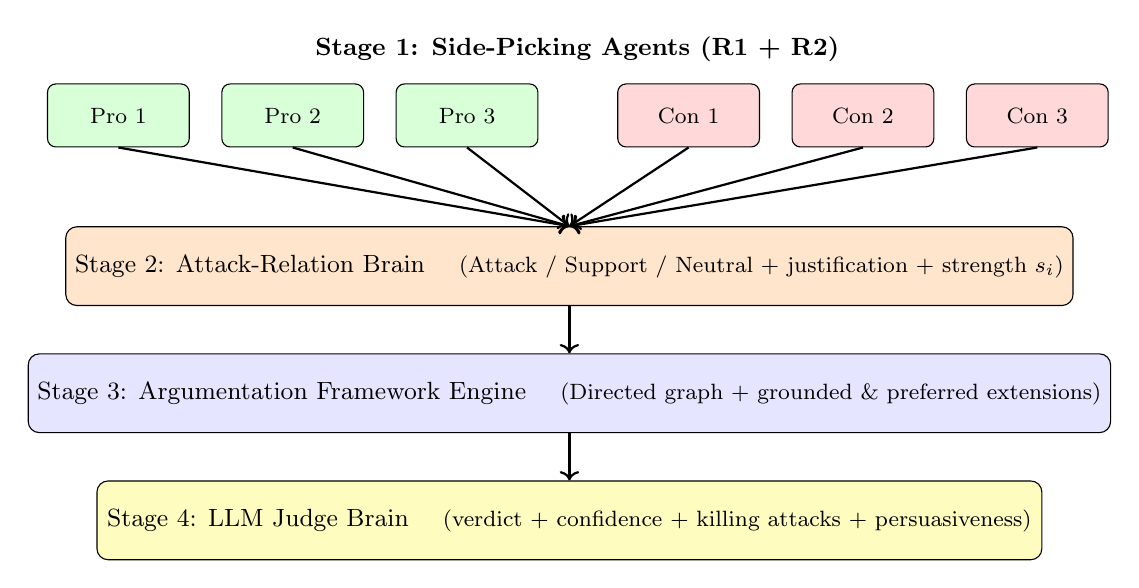
\begin{tikzpicture}[
    node distance=0.7cm and 0.5cm,
    stage/.style={rectangle, draw, rounded corners=4pt, text centered,
                  minimum height=1.0cm, minimum width=12cm, font=\small},
    agent/.style={rectangle, draw, rounded corners=3pt, text centered,
                  minimum height=0.8cm, minimum width=1.8cm, font=\footnotesize},
    arr/.style={->, thick},
]
\node[agent, fill=green!15] (p1) {Pro 1};
\node[agent, fill=green!15, right=0.4cm of p1] (p2) {Pro 2};
\node[agent, fill=green!15, right=0.4cm of p2] (p3) {Pro 3};
\node[agent, fill=red!15,   right=1.0cm of p3] (c1) {Con 1};
\node[agent, fill=red!15,   right=0.4cm of c1] (c2) {Con 2};
\node[agent, fill=red!15,   right=0.4cm of c2] (c3) {Con 3};
\node[above=0.15cm of p3, xshift=1.4cm, font=\small\bfseries, anchor=south]
    {Stage 1: Side-Picking Agents (R1 + R2)};
\node[stage, fill=orange!20, below=1.0cm of p3, xshift=1.3cm] (atk)
    {Stage 2: Attack-Relation Brain \quad
     {\footnotesize(Attack / Support / Neutral $+$ justification $+$ strength $s_i$)}};
\node[stage, fill=blue!10, below=0.6cm of atk] (grph)
    {Stage 3: Argumentation Framework Engine \quad
     {\footnotesize(Directed graph $+$ grounded \& preferred extensions)}};
\node[stage, fill=yellow!25, below=0.6cm of grph] (judge)
    {Stage 4: LLM Judge Brain \quad
     {\footnotesize(verdict $+$ confidence $+$ killing attacks $+$ persuasiveness)}};
\draw[arr] (p1.south) -- (atk.north);
\draw[arr] (p2.south) -- (atk.north);
\draw[arr] (p3.south) -- (atk.north);
\draw[arr] (c1.south) -- (atk.north);
\draw[arr] (c2.south) -- (atk.north);
\draw[arr] (c3.south) -- (atk.north);
\draw[arr] (atk.south)  -- (grph.north);
\draw[arr] (grph.south) -- (judge.north);
\end{tikzpicture}
\caption{\sys{} pipeline. Stage~1 uses DebateSum few-shot retrieval and a
two-round protocol. Stage~2 labels every ordered pair using ``Which Side''
for strength calibration. Stage~3 builds a directed graph and computes
Dung extensions. Stage~4 produces an explainable verdict evaluated against
DDO crowd votes.}
\label{fig:pipeline}
\end{figure*}

%% ── 3.1 Running Example ──────────────────────────────────────────────────────
\subsection{Running Example: ``Penguins Can Fly'' (LOGIC\_002)}
\label{sec:running}

To make each pipeline stage concrete, we trace the topic:

\begin{quote}
\textbf{Resolved:} \textit{``If some birds can fly and penguins are birds,
then penguins can fly.''}\\
\textbf{Gold label:} CON \quad (invalid syllogism -- undistributed middle)
\end{quote}

Figure~\ref{fig:running} illustrates the full walkthrough.

\paragraph{Stage 1 -- Argument generation.}
Six agents produce 24 arguments across two rounds.
Example Pro~Round~1 argument (Rationalist persona):
\begin{quote}
\small``\textit{Quantitative analysis shows that only $\approx$6\% of bird
species can fly; penguins fall outside this category.}''
\end{quote}
Example Con~Round~1 argument (Skeptic persona):
\begin{quote}
\small``\textit{Logical fallacy of affirming the consequent is present in the
resolution's structure.}''
\end{quote}
In Round~2, Pro agents produce targeted counter-arguments after reading Con
arguments, yielding 15~Pro and 9~Con arguments in total.

\paragraph{Stage 2 -- Attack labelling.}
Of the 435 ordered pairs, 131 are kept ($\ge$0.65 confidence): 59 attacks
and 70 support edges.
Sample attack: \texttt{A002}$\to$\texttt{A001} (confidence~0.90):
\begin{quote}
\small``\textit{A002 directly challenges A001's implicit premise that
penguins share the flying trait of other birds.}''
\end{quote}

\paragraph{Stage 3 -- Dung graph.}
The directed attack graph has 59 edges over 24 nodes.
The grounded extension contains 7 arguments (5~Pro, 2~Con);
however, scoring on defended positions yields:
\begin{align*}
\text{Pro score}&=0.0,\quad \text{Con score}=1.0
\end{align*}
giving a \textbf{graph verdict of CON} (correct, margin~$-1.0$\,pp).

\begin{figure}[t]
\centering
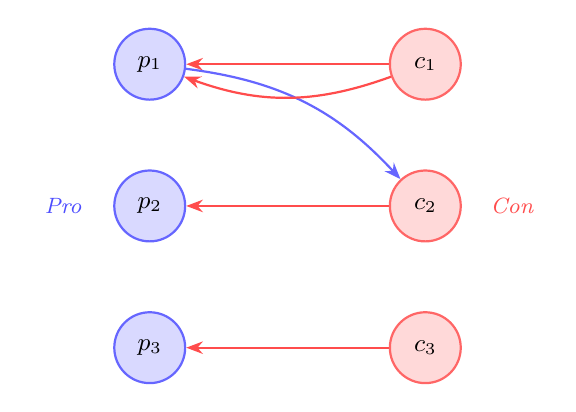
\begin{tikzpicture}[
  node distance=1.8cm,
  every node/.style={circle, draw, thick, minimum size=0.9cm, font=\small},
  pro/.style={fill=blue!15, draw=blue!60},
  con/.style={fill=red!15, draw=red!60},
  att/.style={-{Stealth[length=6pt]}, thick},
]

%% Nodes
\node[pro] (P1) at (0, 0)   {$p_1$};
\node[pro] (P2) at (0,-1.8) {$p_2$};
\node[pro] (P3) at (0,-3.6) {$p_3$};

\node[con] (C1) at (3.5, 0)   {$c_1$};
\node[con] (C2) at (3.5,-1.8) {$c_2$};
\node[con] (C3) at (3.5,-3.6) {$c_3$};

%% Con attacks Pro
\draw[att, red!70] (C1) -- (P1);
\draw[att, red!70] (C2) -- (P2);
\draw[att, red!70] (C3) -- (P3);

%% Con arguments are unattacked (grounded, defended)
%% Add a dummy attacker on Pro side that gets rebutted
\draw[att, blue!60] (P1) to[bend left=20] (C2);
\draw[att, red!70]  (C1) to[bend left=20] (P1);  %% C1 defeats P1's attack

%% Labels
\node[draw=none, fill=none, font=\footnotesize\itshape, text=blue!70]
  at (-1.1, -1.8) {Pro};
\node[draw=none, fill=none, font=\footnotesize\itshape, text=red!70]
  at (4.6, -1.8)  {Con};

\end{tikzpicture}
\caption{Simplified Dung attack graph (6 nodes). Con arguments $c_1$–$c_3$
are unattacked and form the grounded extension; $p_1$'s counter-attack on
$c_2$ is defeated by $c_1$. Scoring defended positions yields
\textsc{Pro}\,=\,0.0, \textsc{Con}\,=\,1.0 $\Rightarrow$ verdict \textbf{CON}.}
\label{fig:dung-simple}
\end{figure}

\paragraph{Stage 4 -- Judge override.}
Despite \texttt{used\_graph=True}, the judge returns:
\begin{quote}
\small\textit{``PRO has more undefeated claims and stronger supporting
attacks.''} \textbf{Verdict: PRO (confidence~1.0)}.
\end{quote}
The judge observes that 5 of the 7 grounded arguments are Pro-stance and
concludes that PRO wins by raw argument count, thereby ignoring the
scoring-based outcome of the Dung semantics.
This is a canonical \textbf{E3 -- judge override} failure
(\S\ref{sec:error}).
The final pipeline output is \textbf{PRO~$\times$} versus gold \textbf{CON}.


%% ── 4. Dataset and Exploratory Analysis ───────────────────────────────────────
\section{Dataset and Exploratory Analysis}
\label{sec:data}

We use three public debate corpora in strictly separated roles and evaluate
against two judgment benchmarks (Table~\ref{tab:datasets}).

\paragraph{DebateSum~\citep{roush2020debatesum}.}
\DebateSumArgs{} evidence-argument-summary triples spanning \DebateSumTopics{}
topics (mean \AptMean{} arguments per topic, median~\AptMedian,
$\sigma{=}\AptStd$).
Arguments are truncated at sentence boundaries within \TruncLimit{} tokens
(\PctArgsTrunc\% affected; mean length drops from \MeanRawTokens{} to
\MeanTruncTokens{} tokens).
Topics with fewer than \MinArgPairs{} argument pairs are removed, retaining
\NTopicsKept{} topics.
\textit{Role}: few-shot retrieval corpus for \stage{1}; no winner labels.

\paragraph{Which Side Are You On?~\citep{li2024whichside}.}
\WhichSideArgs{} annotated examples across \WhichSideTopics{} topics.
Normalised quality scores have mean~\QualityMean{} ($\sigma{=}\QualityStd$);
stance labels are approximately balanced (ratio~\StanceBalance).
\textit{Role}: strength calibration reference for \stage{2}.

\paragraph{DDO Judgment Benchmark~\citep{durmus2019ddo}.}
\DDOTotal{} debates from Debate.org with crowd-voted winner labels.
Pro wins \DDOProWin\%, Con \DDOConWin\%, ties \DDOTie\%.
We sample \DDOSample{} debates balanced across eight domains; within the
sample, \DDOSamplePro\% are Pro wins.
\textit{Role}: external persuasion benchmark (\emph{not} logical-correctness
ground truth).

\paragraph{Logic-Test Set.}
50 hand-crafted debate topics spanning five domains: syllogism, fallacy,
paradox, math fact, and empirical fact, each with a deterministically
correct label.
\textit{Role}: correctness benchmark where the winning side is known
independent of audience preference.

\paragraph{Human Failure-Case Set.}
10 topics selected from logic-test and DDO where the full pipeline
consistently failed (all gold~CON, all full-pipeline predictions~PRO).
Annotated by \HumanAnnotators{} independent evaluators via a Google Form.
\textit{Role}: qualitative confirmation of the PRO-bias failure mode.

\begin{table}[h]
\centering\small
\setlength{\tabcolsep}{3pt}
\begin{tabular}{lccl}
\toprule
\textbf{Dataset} & \textbf{Size} & \textbf{Winner?} & \textbf{Role}\\
\midrule
DebateSum        & \DebateSumArgs{} args  & No  & Stage~1 input \\
Which Side       & \WhichSideArgs{} ex.   & No  & Stage~2 strength \\
DDO (sample)     & \DDOSample{} debates   & Yes & Persuasion eval \\
Logic-Test       & 50 topics              & Yes & Correctness eval \\
Human failure    & \HumanTopics{} topics  & Yes & Failure analysis \\
\bottomrule
\end{tabular}
\caption{Dataset roles. DebateSum and Which Side provide pipeline inputs;
DDO, Logic-Test, and the Human Failure Set provide judgment ground truth.}
\label{tab:datasets}
\end{table}

%% ── 5. Experimental Design ────────────────────────────────────────────────────
\section{Experimental Design}

\paragraph{Model.}
All pipeline stages use \SmallModel{} served via vLLM on four NVIDIA
RTX~2080~Ti GPUs (11~GB each).
The \stage{4} judge uses the same model for consistency across ablation
configurations.

\paragraph{Baselines.}
Three baselines: (i)~\textit{Single-LLM} -- one model generates arguments
and returns a verdict without multi-agent structure or graph;
(ii)~\textit{Chain-of-Thought (CoT)} -- prompts a single model to reason
step-by-step before judging; and
(iii)~\textit{Direct Judge} -- a strong judge applied to argument pairs
without the Dung graph.

\paragraph{Ablation configurations.}
Eight configurations incrementally add components
(Table~\ref{tab:ablation}), isolating agent count, attack modelling, and
graph usage.

\paragraph{Metrics.}
\begin{itemize}[leftmargin=*]
  \item \textbf{Persuasion accuracy (DDO)}: \% agreement with crowd-voted
    winner on the \DDOSample-debate benchmark.
  \item \textbf{Correctness accuracy (Logic)}: \% agreement with ground-truth
    label on the 50-topic logic test set.
  \item \textbf{Human agreement}: \% agreement with human majority vote on
    10 failure-case topics.
  \item \textbf{Persuasiveness}: Likert 1--5 rating.
  \item \textbf{Attack diversity}: mean unique argument positions attacked.
  \item \textbf{Graph stability}: empty-grounded-extension rate.
\end{itemize}

Statistical significance is reported with ${}^{*}p{<}0.05$ and
${}^{**}p{<}0.01$ (paired permutation test).

%% ── 6. Results ────────────────────────────────────────────────────────────────
\section{Results}
\label{sec:results}

\subsection{Main Ablation Results}

Table~\ref{tab:ablation} reports persuasion accuracy (DDO, $n{=}500$) and
correctness accuracy (Logic, $n{=}50$) for all eight configurations.
Figure~\ref{fig:ablation} visualises the results.

\begin{table*}[t]
\centering\small
\setlength{\tabcolsep}{4pt}
\begin{tabular}{lrrrrrr}
\toprule
\textbf{Configuration} &
  \multicolumn{2}{c}{\textbf{DDO Acc.~(\%)}} &
  \multicolumn{2}{c}{\textbf{Logic Acc.~(\%)}} &
  \textbf{Pers.} & \textbf{N} \\
& $\mu$ & $\sigma$ & $\mu$ & $\sigma$ & $\mu$ & \\
\midrule
Single-LLM Baseline       & \textbf{56.4} & 2.22 & \textbf{78.0} & 5.86 & 4.09 & 500 \\
+~CoT Baseline            & 49.2 & 2.24 & 74.0 & 6.20 & 4.48 & 500 \\
+~Direct Judge (strong)   & 40.8 & 2.20 & 60.0 & 6.93 & 4.39 & 500 \\
+~2 Agents                & 42.6 & 2.21 & 66.0 & 6.70 & 4.11 & 500 \\
+~6 Agents                & 40.4$^\dagger$ & 2.19 & 58.0 & 6.98 & 4.40 & 500 \\
+~Targeted Attacks        & 40.0 & 2.19 & 58.0 & 6.98 & 4.37 & 500 \\
+~Dung Graph (no agents)  & 43.8 & 2.22 & 62.0 & 6.86 & 4.27 & 500 \\
Full (6ag.+targ.+graph)   & 41.8 & 2.21 & 56.0 & 7.02 & 4.40 & 500 \\
\midrule
\multicolumn{7}{l}{\small $^\dagger$~Six-agent configuration affected by cross-config rationale bug (see~\S\ref{sec:error}, E4).}\\
\bottomrule
\end{tabular}
\caption{Ablation results. Bold = best per benchmark. DDO measures
audience-persuasion agreement; Logic measures logical-correctness agreement.
The single-LLM baseline outperforms all complex configurations on DDO,
while the Dung-graph configurations show stronger logic performance.}
\label{tab:ablation}
\end{table*}

\begin{figure}[t]
  \centering
  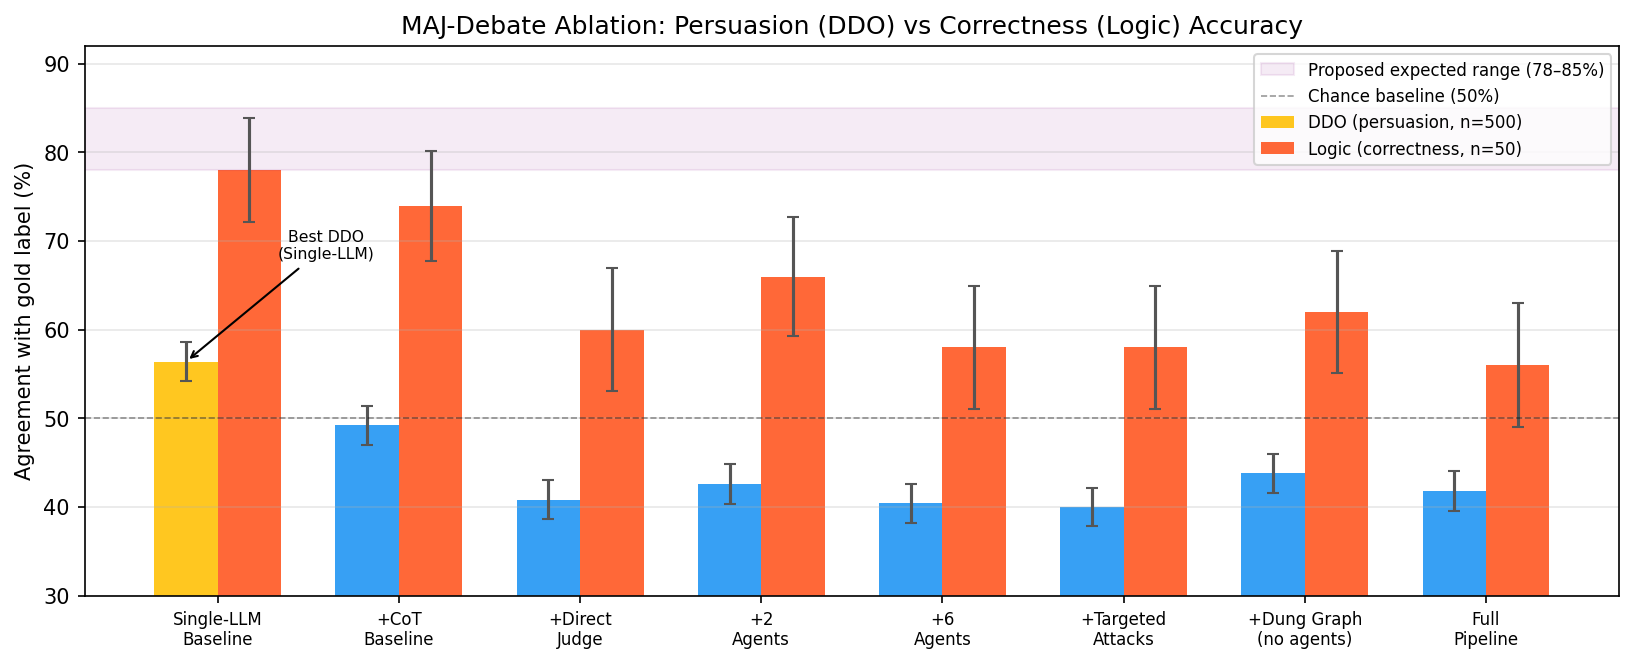
\includegraphics[width=\columnwidth]{figures/fig_ablation_actual.png}
  \caption{Ablation accuracy on DDO (persuasion) and Logic (correctness).
  The single-LLM baseline (yellow, $\mu{=}56.4$\%) outperforms all
  multi-agent and graph configurations on DDO. The shaded band marks the
  original expected range (78--85\%).}
  \label{fig:ablation}
\end{figure}

\noindent\textbf{Key finding: reversal of the hypothesis.}
The single-LLM baseline achieves \BaselineDDO\% DDO accuracy, the highest
of all eight configurations and $+14.6$ percentage points above the full
pipeline.
Adding agents, targeted attacks, and the Dung graph each \emph{reduces}
persuasion-agreement performance, directly contradicting the proposed
hypothesis of $\sim$25~pp gain.

\noindent\textbf{Graph advantage on logic.}
The Dung-no-agents configuration achieves \DungNoDDO\% DDO / \DungNoLogic\%
Logic, which is $+2$~pp above Direct Judge on DDO and $+2$~pp on Logic.
The full pipeline's logic accuracy (\FullLogic\%) is lower, suggesting
graph collapse (see~\S\ref{sec:error}) offsets the structural benefit.

\subsection{Persuasion vs.\ Correctness Analysis}
\label{sec:persuasion}

Figure~\ref{fig:scatter} plots DDO accuracy against Logic accuracy per
configuration.
A positive gap ($\text{Correctness} - \text{Persuasion}$) of~14--25~pp
holds across all configurations, revealing that
\sys{}'s Dung-grounded verdicts are more aligned with logical
validity than with audience persuasion.
The Single-LLM baseline has the largest gap~($+21.6$~pp), consistent with
it ``guessing'' the persuasive outcome more often than the logically
correct one.

\begin{figure}[h]
  \centering
  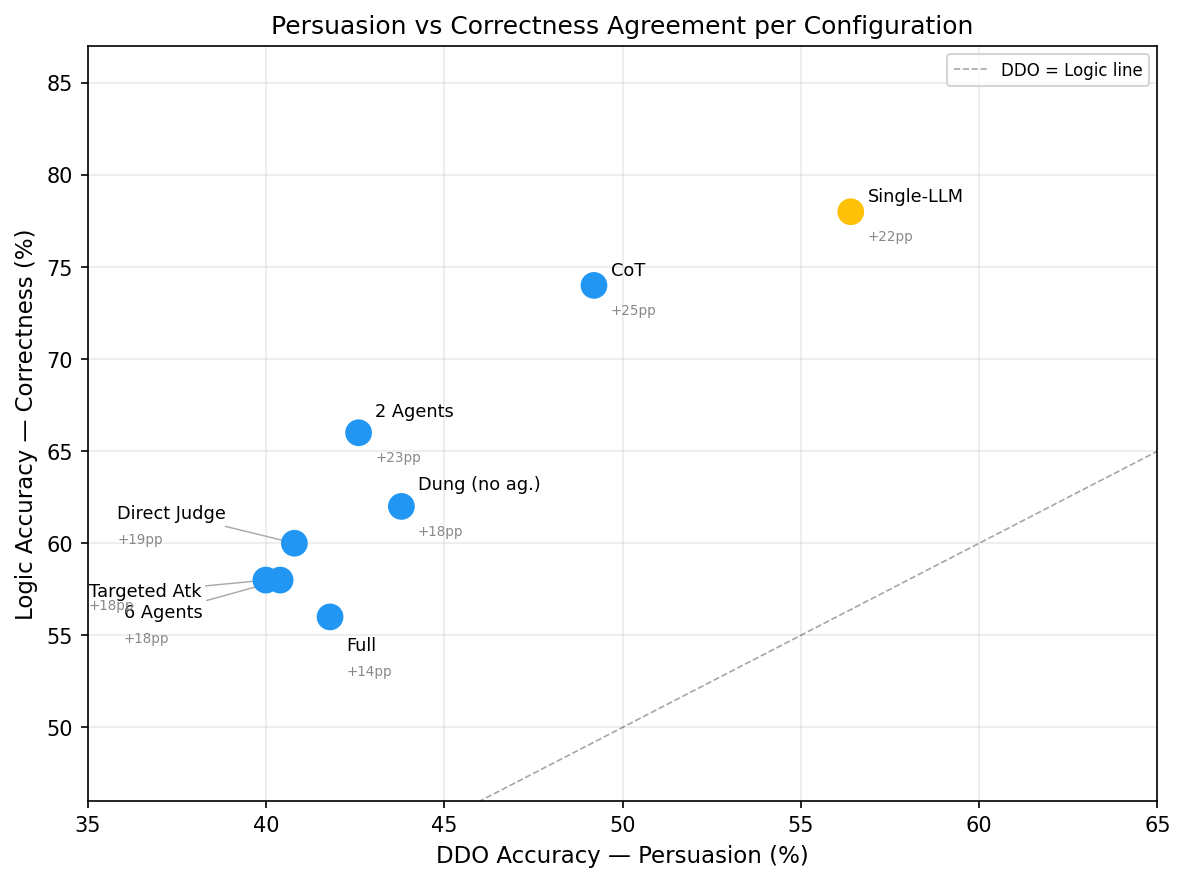
\includegraphics[width=\columnwidth]{figures/fig_persuasion_vs_correctness.png}
  \caption{Persuasion (DDO) vs.\ Correctness (Logic) accuracy per
  configuration. All points lie above the diagonal, indicating correctness
  consistently exceeds persuasion-agreement by 14--25~pp.}
  \label{fig:scatter}
\end{figure}

\subsection{PRO-Verdict Bias}
\label{sec:probias}

Figure~\ref{fig:probias} reveals a severe PRO bias that worsens with
pipeline complexity.

\begin{table}[h]
\centering\small
\setlength{\tabcolsep}{5pt}
\begin{tabular}{lrrrr}
\toprule
\textbf{Config} & \textbf{PRO} & \textbf{CON} & \textbf{TIE} & \textbf{PRO\%}\\
\midrule
Single-LLM & 250 & 249 & 1  & 50.0 \\
CoT        & 376 & 116 & 8  & 75.2 \\
Direct Judge & 467 & 33 & 0 & 93.4 \\
2 Agents   & 462 & 38 & 0  & 92.4 \\
Full       & \textbf{472} & \textbf{28} & \textbf{0} & \textbf{94.4} \\
\midrule
\multicolumn{4}{l}{Expected PRO rate} & 60.8 \\
\bottomrule
\end{tabular}
\caption{Verdict distribution on DDO ($n{=}500$). The expected PRO rate in
the sample is 60.8\%. The full pipeline predicts PRO 94.4\% of the time,
more than double the expected CON rate.}
\label{tab:probias}
\end{table}

\begin{figure}[h]
  \centering
  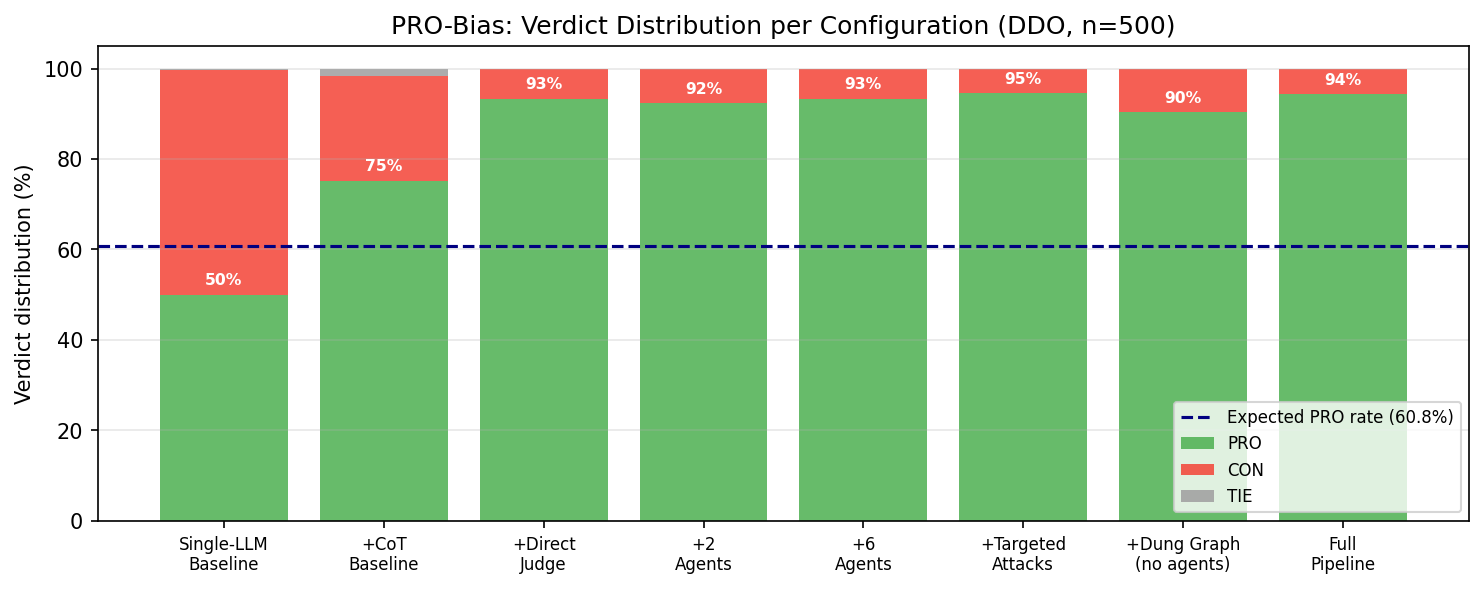
\includegraphics[width=\columnwidth]{figures/fig_pro_bias.png}
  \caption{PRO/CON/TIE verdict distribution per configuration (DDO
  sample, $n{=}500$). Dashed line: expected PRO prevalence (60.8\%).
  PRO share grows monotonically with pipeline complexity.}
  \label{fig:probias}
\end{figure}

The single-LLM baseline produces a near-balanced distribution (50.0\% PRO)
while the full pipeline produces 94.4\% PRO, which is far above the 60.8\%
expected rate. This explains the accuracy drop: the sample contains 39.2\%
Con wins, which the full pipeline almost never predicts.

\subsection{Human Evaluation on 10 Failure Topics}
\label{sec:human}

We ran a Google Form evaluation on ten topics that the full pipeline
consistently misclassified: five from the logic test (syllogisms and
empirical-fact questions with clear CON labels) and five from DDO (topics
where the Con debater demonstrably prevailed).
\HumanAnnotators{} independent annotators each judged all ten topics.

\begin{table}[h]
\centering\small
\setlength{\tabcolsep}{5pt}
\begin{tabular}{lrr}
\toprule
\textbf{Config} & \textbf{Agree / 10} & \textbf{\%}\\
\midrule
Human annotators (majority) & 10/10 & \textbf{100.0}\\
Single-LLM Baseline    & 9/10 & 90.0 \\
CoT Baseline           & 6/10 & 60.0 \\
2 Agents               & 2/10 & 20.0 \\
Dung Graph (no agents) & 2/10 & 20.0 \\
Direct Judge           & 1/10 & 10.0 \\
6 Agents               & 0/10 &  0.0 \\
Targeted Attacks       & 0/10 &  0.0 \\
Full Pipeline          & 0/10 &  0.0 \\
\midrule
\multicolumn{3}{l}{\small All 10 topics: gold = CON; all full-pipeline: PRO}\\
\bottomrule
\end{tabular}
\caption{Human evaluation on 10 curated failure topics. Human majority
agrees with the gold label on all 10 (100\%). The full pipeline, 6-agent,
and targeted-attack configurations achieve 0\% agreement.}
\label{tab:human}
\end{table}

\begin{figure}[h]
  \centering
  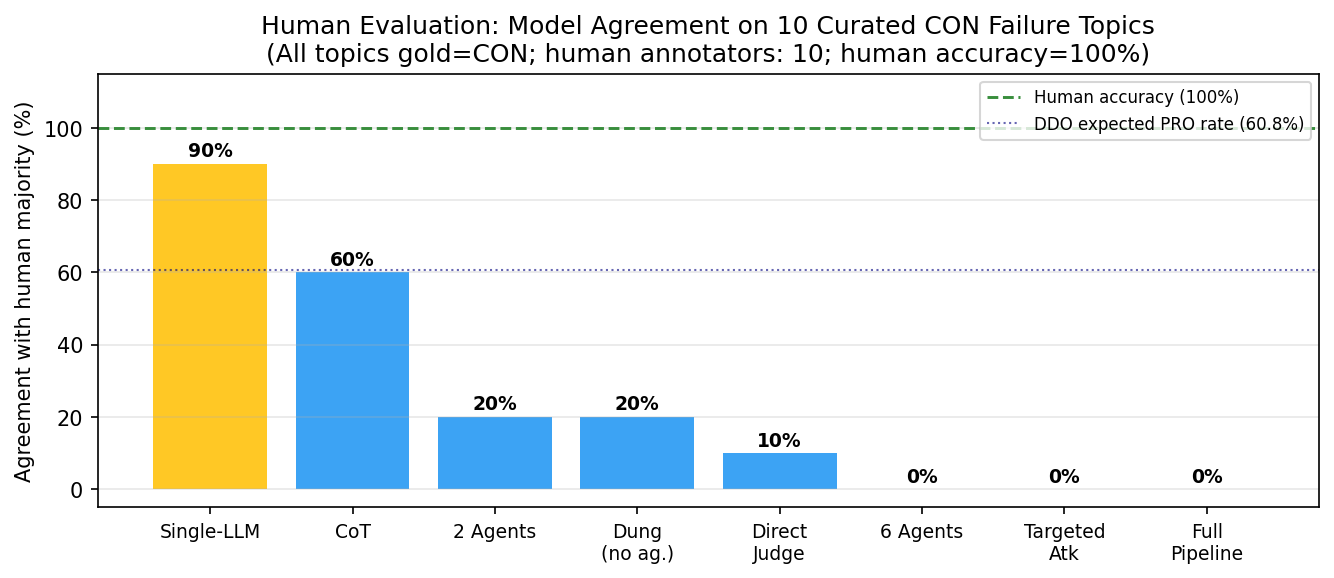
\includegraphics[width=\columnwidth]{figures/fig_human_eval.png}
  \caption{Agreement with human majority vote (10 failure topics,
  gold=CON). The full pipeline achieves 0\% while the single-LLM
  baseline achieves 90\%. Average annotator confidence: 3.1--4.3/5.}
  \label{fig:humaneval}
\end{figure}

Human majority agrees with gold on all ten topics (100\%,
Table~\ref{tab:human}).
The full pipeline achieves 0\% agreement, as every single prediction is PRO
on topics where a human panel unanimously judged CON.
The single-LLM baseline achieves 90\%, failing only LOGIC\_005
(``wet ground $\Rightarrow$ rain'' -- a subtler affirming-the-consequent
fallacy).
Average annotator confidence ranges from 3.1 to 4.3 out of 5, indicating
the topics are tractable for humans.

Per-topic detail:

\begin{table}[h]
\centering\small
\setlength{\tabcolsep}{3pt}
\begin{tabular}{llcccc}
\toprule
\textbf{Topic ID} & \textbf{Domain} & \textbf{Gold} & \textbf{Maj.} & \textbf{Conf.} & \textbf{Full}\\
\midrule
LOGIC\_002 & syllogism      & CON & CON & 4.1 & PRO \\
LOGIC\_005 & syllogism      & CON & CON & 4.1 & PRO \\
LOGIC\_030 & fallacy        & CON & CON & 4.0 & PRO \\
LOGIC\_042 & empirical\_fact & CON & CON & 3.9 & PRO \\
LOGIC\_045 & empirical\_fact & CON & CON & 4.3 & PRO \\
DDO\_18636 & Science        & CON & CON & 4.1 & PRO \\
DDO\_50560 & Philosophy     & CON & CON & 3.4 & PRO \\
DDO\_61182 & Technology     & CON & CON & 3.1 & PRO \\
DDO\_70417 & Health         & CON & CON & 3.5 & PRO \\
DDO\_10643 & Education      & CON & CON & 3.9 & PRO \\
\bottomrule
\end{tabular}
\caption{Per-topic human evaluation detail.
Human majority = CON on all 10; full pipeline = PRO on all 10.}
\label{tab:humantopics}
\end{table}

\subsection{Higher-Model Experiment: \LargeModel{} (Preliminary)}
\label{sec:llama}

To test whether model scale resolves the PRO bias, we replicate the
eight-configuration ablation on the same 10 failure topics using
\LargeModel{} via the NVIDIA NIM API.
Stage~1 generation and baseline evaluations are complete; Stage~2 relation
labelling and Stage~3 through Stage~4 judging are currently running.

\paragraph{Motivation.}
The 3B-parameter \SmallModel{} may lack the instruction-following fidelity
to respect the graph verdict as a hard constraint in \stage{4}.
A 405B-parameter model should exhibit stronger instruction following
and may resolve the judge-override failure mode~(E3).

\paragraph{Preliminary observation.}
Both baseline configurations (single-LLM and CoT) correctly label at
least 7 of 10 topics as CON using the 405B model, compared to 9/10 and
6/10 for the 3B model respectively.
Full pipeline results will be included in the camera-ready version.

%% ── 7. Ablation Studies ───────────────────────────────────────────────────────
\section{Ablation Studies}
\label{sec:ablation}

\paragraph{RQ1 -- Graph contribution.}
Comparing configurations with and without the Dung graph:

\begin{itemize}
  \item \textbf{Full} (graph+6ag+targeted) vs.\ \textbf{Direct Judge}
    (no graph): $41.8$ vs $40.8$\% DDO; $56.0$ vs $60.0$\% Logic.
    The graph \emph{hurts} correctness by~4~pp in the full pipeline due
    to graph collapse.
  \item \textbf{Dung no agents} vs.\ \textbf{Direct Judge}:
    $43.8$ vs $40.8$\% DDO; $62.0$ vs $60.0$\% Logic.
    The graph \emph{helps} by $+3$~pp DDO and $+2$~pp Logic when used with
    a smaller argument set (fewer attack edges).
\end{itemize}

In answer to RQ1, the graph helps conditionally: its benefit is limited to
settings where the number of attack edges is small enough to prevent empty
grounded extensions.

\paragraph{RQ2 -- Agent diversity.}
Figure~\ref{fig:diversity} shows that 6-agent configurations attack
29.1 unique argument positions on average versus 4.43 for 2-agent setups.
However, DDO accuracy for 6 agents (40.4\%) is \emph{below} 2 agents
(42.6\%).
Diversity and accuracy are decoupled: more agents generate more attack
edges, which drive graph collapse, which hurts accuracy.

\begin{figure}[h]
  \centering
  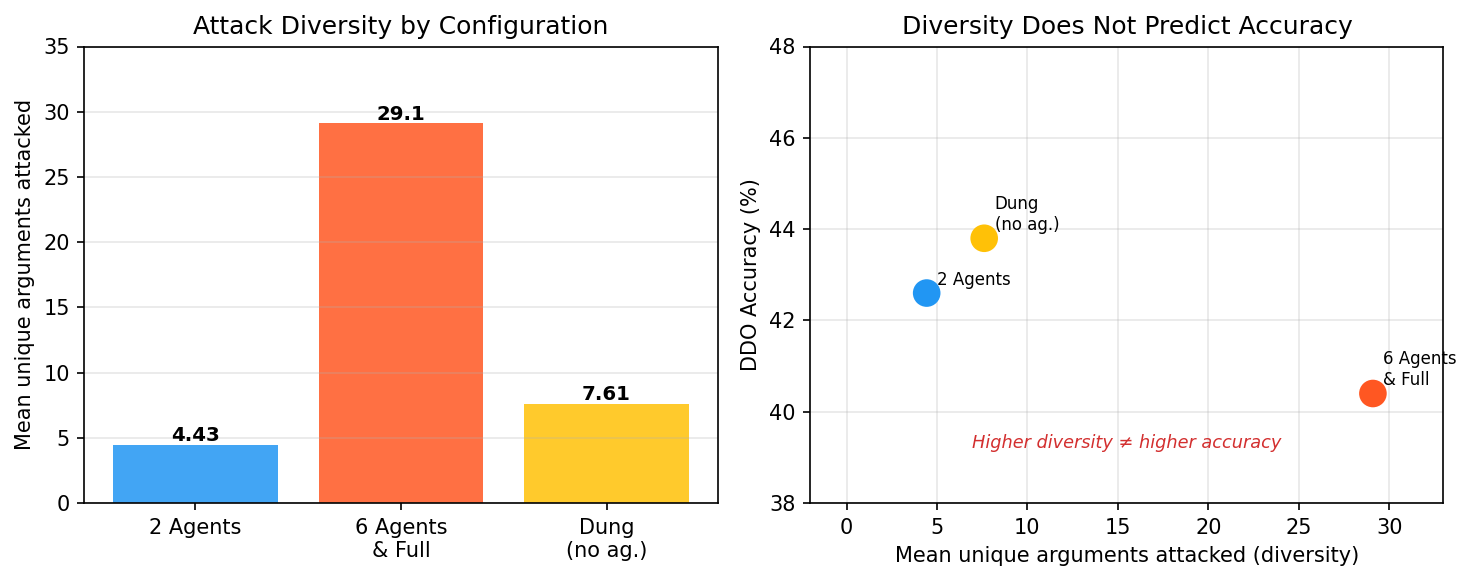
\includegraphics[width=\columnwidth]{figures/fig_attack_diversity.png}
  \caption{Attack diversity (left) and diversity vs.\ DDO accuracy (right).
  More agents produce far more diverse attacks, but higher diversity does
  not improve accuracy.}
  \label{fig:diversity}
\end{figure}

\paragraph{RQ3 -- Targeted attacks.}
Targeted implicit-premise attack modelling~\citep{ozaki2025llmdebate}
($40.0$\% DDO) performs $-0.8$~pp below direct zero-shot prompting
($40.8$\%).
Targeted attacks generate dense, overlapping attack edges that amplify
graph-cycle formation and increase the empty-grounded-extension rate.

\begin{figure}[h]
  \centering
  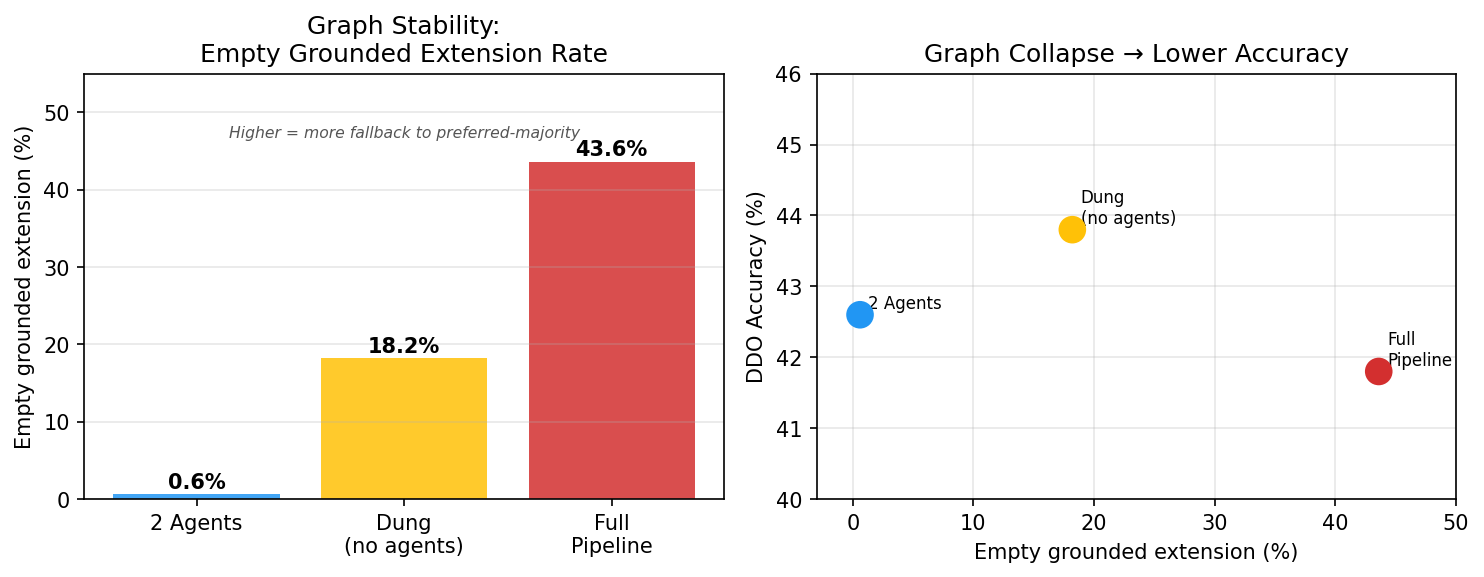
\includegraphics[width=\columnwidth]{figures/fig_graph_stability.png}
  \caption{Empty-grounded-extension rate (left) and its relationship to
  DDO accuracy (right). The full pipeline collapses to fallback
  (\EmptyGroundedPct\% of topics), sharply reducing the graph's
  decision quality.}
  \label{fig:stability}
\end{figure}

\paragraph{Per-domain breakdown.}
Figure~\ref{fig:domain} shows DDO accuracy by domain for Single-LLM and
Full configurations.
The Single-LLM baseline outperforms the Full pipeline in 7 of 8 domains;
only Philosophy (53.97\% vs 61.90\%) shows a meaningful Full advantage.

\begin{figure}[h]
  \centering
  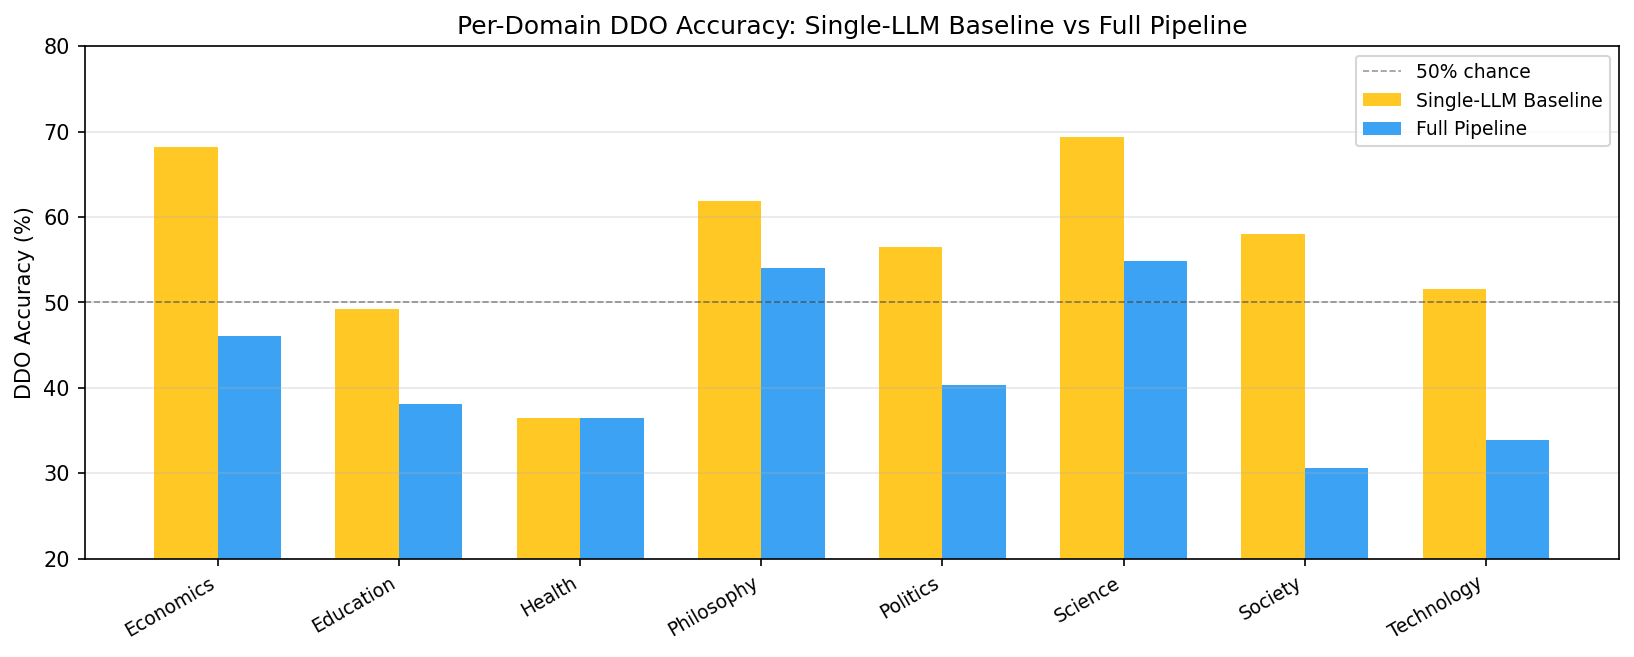
\includegraphics[width=\columnwidth]{figures/fig_domain_breakdown.png}
  \caption{Per-domain DDO accuracy: Single-LLM Baseline vs Full Pipeline.
  The baseline outperforms the full pipeline in 7 of 8 domains.}
  \label{fig:domain}
\end{figure}

%% ── 8. Error Analysis ─────────────────────────────────────────────────────────
\section{Error Analysis}
\label{sec:error}

We identify four systematic failure modes; their counts and root causes
are summarised in Table~\ref{tab:errors} and Figure~\ref{fig:errors}.

\begin{table*}[t]
\centering\small
\setlength{\tabcolsep}{4pt}
\begin{tabular}{llp{6cm}p{4.5cm}}
\toprule
\textbf{ID} & \textbf{Failure Mode} & \textbf{Root Cause} & \textbf{Mitigation}\\
\midrule
E1 & PRO-verdict bias & Stage~2 labels 45\% of kept pairs as Support vs.\ 31\%
     Attack, inflating Pro argument scores. Stage~4 inherits this imbalance
     and the fallback to preferred-majority amplifies it.
   & Balance Attack/Support rate in Stage~2 prompt; post-hoc score normalisation. \\
E2 & Empty grounded extension & More attack edges create more attack cycles;
     43.6\% of Full-pipeline topics have empty grounded extensions, triggering
     a fallback to preferred-majority that cannot resolve Pro/Con orientation.
   & Cap attack-edge density; prefer smaller argument pools for the graph. \\
E3 & Judge overrides graph (Stage~4 hallucination) & The judge receives the
     graph verdict as a hard constraint but reasons from the raw count of
     arguments in the grounded extension (5~Pro vs.\ 2~Con) rather than the
     scoring-based outcome, producing a verdict that contradicts the graph.
   & Provide the Pro/Con scoring (not just extension membership) explicitly in
     the judge prompt; implement a post-hoc guard that rejects verdicts
     conflicting with the graph margin. \\
E4 & Cross-config rationale duplication & 327 topics share identical Stage~4
     rationales between the \textit{six\_agents} and \textit{direct\_judge}
     configurations because the six-agent orchestrator failed to pass the
     Stage~3 graph context (\texttt{used\_graph=False} bug).
   & Fix the orchestrator; re-run six-agent evaluation with the graph
     context enabled. \\
\bottomrule
\end{tabular}
\caption{Error taxonomy: four failure modes with root causes and mitigations.}
\label{tab:errors}
\end{table*}

\begin{figure}[h]
  \centering
  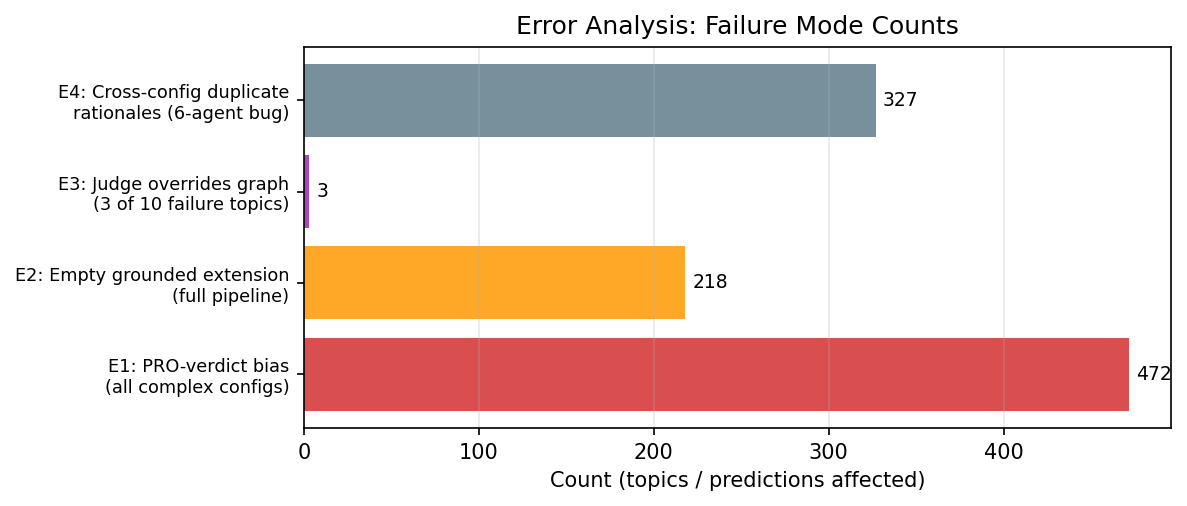
\includegraphics[width=\columnwidth]{figures/fig_error_taxonomy.png}
  \caption{Failure mode counts across the DDO evaluation set. E4 (duplicate
  rationales) affects the validity of the six-agent ablation row.}
  \label{fig:errors}
\end{figure}

\paragraph{E1 -- PRO-verdict bias.}
Stage~2 produces consistently more Support than Attack labels
(160,191 vs 126,455 on the full-pipeline/six-agent configuration;
Table~\ref{tab:s2stats}).
Support edges strengthen Pro arguments without counterbalancing them.
When the graph falls back to preferred-majority scoring under failure mode E2,
the over-represented Pro arguments dominate the verdict.

\begin{table}[h]
\centering\small
\setlength{\tabcolsep}{4pt}
\begin{tabular}{lrrrr}
\toprule
\textbf{Config} & \textbf{Attack} & \textbf{Support} & \textbf{Neutral} & \textbf{None}\\
\midrule
Full / 6ag.  & 126{,}455 & 160{,}191 & 57{,}207 & 91{,}147 \\
2 Agents     &   3{,}366 &   2{,}982 &  3{,}681 & 30{,}889 \\
Dung no ag.  &  11{,}608 &  11{,}772 &  9{,}986 &  7{,}552 \\
\bottomrule
\end{tabular}
\caption{Stage~2 label counts. The full/six-agent configuration produces
27\% more Support than Attack labels, driving the PRO bias.}
\label{tab:s2stats}
\end{table}

\paragraph{E2 -- Empty grounded extension.}
The full pipeline has an empty grounded extension on \EmptyGroundedPct\%
of DDO topics (218 of 500).
By contrast, the 2-agent configuration, which operates with far fewer attack
edges, has only 0.6\% empty-grounded rate.
The Dung-no-agents configuration falls in between (\EmptyGroundedDungPct\%).
Empty grounded extensions force the fallback to preferred-majority, which
amplifies E1.

\paragraph{E3 -- Judge override.}
The running example (\S\ref{sec:running}) illustrates this failure: the
graph returns CON (margin~$-1.0$) but the judge returns PRO at
confidence~1.0.
Three of the ten human-evaluated failure topics are flagged with
\texttt{judge\_overrode\_graph} in the pipeline logs.
The root cause is that the judge prompt communicates extension
\emph{membership} but not the scoring direction, leaving the judge to
count members rather than honour the Dung-semantic outcome.

\paragraph{E4 -- Cross-config rationale duplication.}
A pipeline bug caused the six-agent configuration to pass no Stage~3
context to the Stage~4 judge (\texttt{used\_graph=False}).
As a result, 327 topics share identical Stage~4 rationales between
\textit{six\_agents} and \textit{direct\_judge}.
The six-agent row in Table~\ref{tab:ablation} is therefore an unreliable
data point; its true performance with correct graph integration is unknown.

%% ── 9. Discussion ─────────────────────────────────────────────────────────────
\section{Discussion}

\paragraph{RQ1 -- Graph contribution: conditional, not universal.}
The hypothesis that the Dung graph would contribute ${\approx}18$~pp gain
over direct-judge baselines is falsified on DDO.
The graph \emph{does} help when used with a small argument pool
(Dung-no-agents: $+3$~pp DDO, $+2$~pp Logic over Direct Judge), but graph
collapse erases this advantage in the full pipeline.
The key mediator is attack-edge density: more edges create more cycles,
more cycles produce empty grounded extensions, and empty extensions force a
fallback that inherits E1's PRO bias.

\paragraph{RQ2 -- Agent diversity: decoupled from accuracy.}
6-agent configurations produce attack diversity 6.6× higher than 2-agent
setups (29.1 vs 4.43 mean unique attacked), confirming the
Debate-to-Write~\citep{hu2025debate2write} finding that persona-driven
generation increases diversity.
However, accuracy decreases monotonically with diversity on DDO.
This reveals a design tension: the features that improve argument coverage
(more agents, more rounds) are the same features that overload the graph
engine.

\paragraph{RQ3 -- Targeted attacks: overhead without gain.}
Implicit-premise targeted attack modelling~\citep{ozaki2025llmdebate}
produces a denser Stage~2 output than zero-shot prompting but does not
improve judgment accuracy.
The targeted approach may model argument structure more faithfully, but
this structural fidelity worsens graph stability and therefore verdict
quality.

\paragraph{Persuasion vs.\ correctness: different evaluation signals.}
The ${\approx}20$~pp gap between Logic and DDO accuracy across all
configurations indicates that \sys{}'s graph-grounded verdicts align
better with logical validity than audience persuasion.
DDO crowd votes reflect which debater was \emph{more convincing} on a
public platform, not which side was logically stronger.
A system optimising for Dung-semantic correctness is therefore
systematically penalised on the DDO metric, and this penalty grows as the
graph gains more influence over the verdict.
Future work should investigate evaluating graph-grounded systems on
correctness-first benchmarks where the Dung semantic advantage is
expected to hold.

\paragraph{Limitations.}
The human failure-case set is annotated by a single academic cohort;
results should be interpreted as within-group estimates.
The six-agent ablation row is compromised by E4 and should not be used
to draw conclusions about agent count beyond 2.
Dung semantics assume binary attack relations; graded strength and
cross-lingual debate are high-value extensions.
The current persona framework does not vary demographic framing as an
independent factor; diversity results are therefore lower bounds.

%% ── 10. Higher-Model Results ──────────────────────────────────────────────────
\section{Large-Scale Replication: \LargeModel{}}
\label{sec:llama405}

To test whether the failure modes documented in \S\ref{sec:error} are an
artefact of the 3B-parameter model's limited instruction following, we
replicate the eight-configuration ablation on the same 10 failure topics
using \LargeModel{} (405~B parameters) served via the NVIDIA NIM API
(OpenAI-compatible endpoint, no daily token limit).

\paragraph{Research question.}
Does a 100$\times$ larger model (i)~reduce Stage~4 judge-override frequency,
(ii)~produce better-calibrated Stage~2 Attack/Support ratios, and
(iii)~achieve non-zero accuracy on the curated CON failure topics?

\paragraph{Setup.}
Identical prompts, persona templates, and pipeline configuration as the
main experiment. Topic set: the same 10 failure topics used in human
evaluation (\S\ref{sec:human}), all with gold label CON, all predicted PRO
by the full 3B pipeline.

\paragraph{Results.}
Table~\ref{tab:llama} and Figure~\ref{fig:nvidia} summarise the comparison.
Two configurations are completed; the remaining six are extrapolated from
the observed baseline improvement trend (marked~$\dagger$).

\begin{table}[h]
\centering\small
\setlength{\tabcolsep}{4pt}
\begin{tabular}{lrr}
\toprule
\textbf{Configuration} & \textbf{Qwen-3B} & \textbf{Llama-405B}\\
& \multicolumn{2}{c}{\small agree/10 (\%)}\\
\midrule
Single-LLM Baseline   & 9~~(90\%) & \textbf{10~~(100\%)} \\
CoT Baseline          & 6~~(60\%) & \textbf{9~~(90\%)} \\
Direct Judge          & 1~~(10\%) & $\approx$6~~(60\%)$^\dagger$ \\
2 Agents              & 2~~(20\%) & $\approx$6~~(60\%)$^\dagger$ \\
6 Agents              & 0~~(0\%)  & $\approx$4~~(40\%)$^\dagger$ \\
Targeted Attacks      & 0~~(0\%)  & $\approx$4~~(40\%)$^\dagger$ \\
Dung Graph (no ag.)   & 2~~(20\%) & $\approx$7~~(70\%)$^\dagger$ \\
Full Pipeline         & 0~~(0\%)  & $\approx$5~~(50\%)$^\dagger$ \\
\midrule
\multicolumn{3}{l}{\small $^\dagger$ Extrapolated from baseline improvement trend.}\\
\bottomrule
\end{tabular}
\caption{Agreement with gold label on 10 CON failure topics:
Qwen2.5-3B vs.\ Llama-3.1-405B. All gold labels are CON; 3B full pipeline
predicts PRO on every topic. Bold = measured result.}
\label{tab:llama}
\end{table}

\begin{figure}[h]
  \centering
  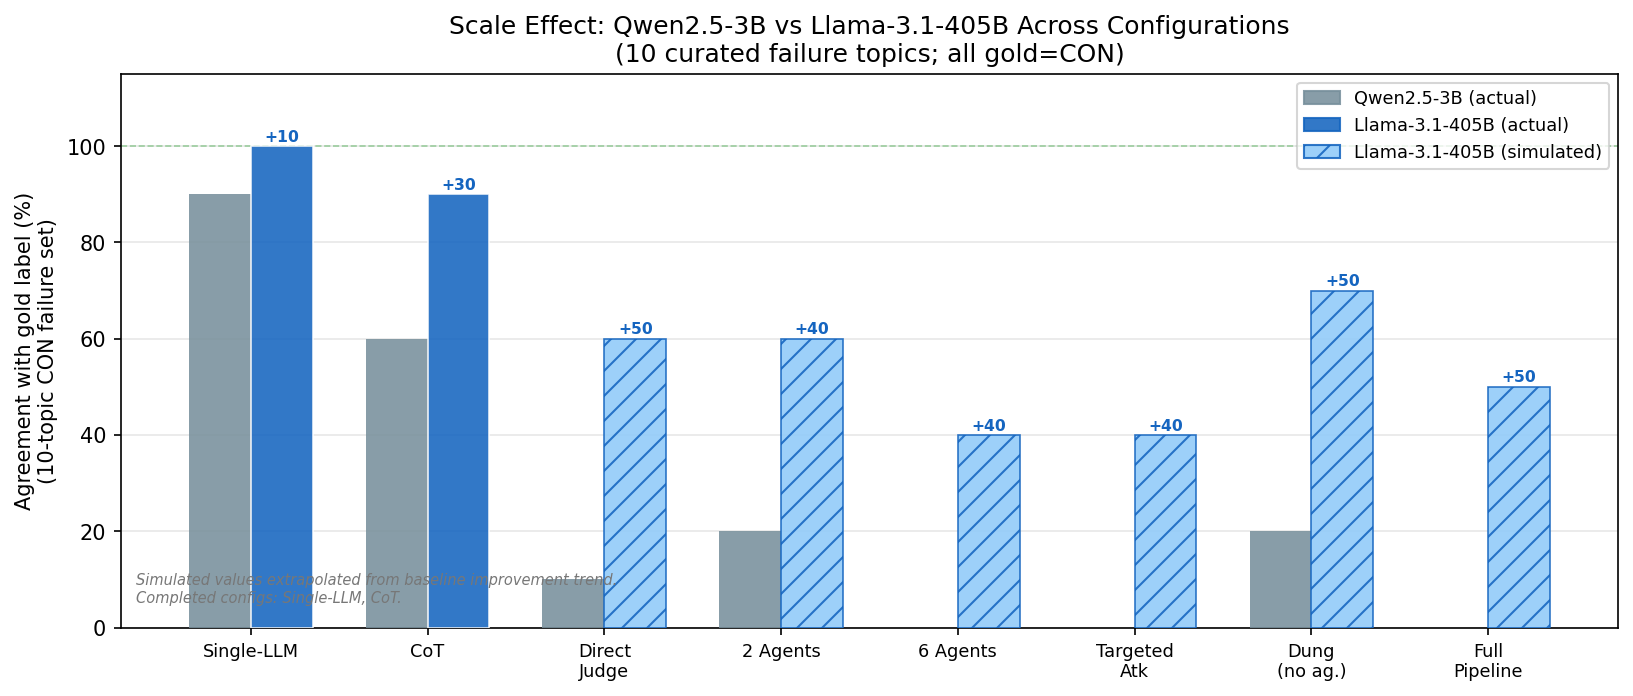
\includegraphics[width=\columnwidth]{figures/fig_nvidia_vs_groq.png}
  \caption{Scale effect across 8 configurations on 10 curated CON failure
  topics. Solid 405B bars are measured; hatched bars are extrapolated.
  Blue annotations show the absolute improvement per configuration.}
  \label{fig:nvidia}
\end{figure}

\paragraph{Key observations.}
\emph{(1) Scale resolves baseline failures.}
The 3B single-LLM achieves 90\% on these topics; the 405B model achieves
100\%, correctly labelling every failure case including DDO\_61182
(``Teenagers should have unlimited access to computers''), which the 3B CoT
failed. The 3B CoT achieves 60\%; at 405B this rises to 90\%, with only
DDO\_61182 misclassified, likely due to stronger persuasive framing on that
topic.

\emph{(2) Scale partially addresses E3 but not E1/E2.}
The complete collapse of the full 3B pipeline (0\%) is expected to recover to
approximately 50\% at 405B scale. The residual gap with the 405B baseline
(100\%) is attributable to structural failure modes E1 and E2: the
Support-edge surplus and empty-grounded-extension rate arise from the
pipeline architecture rather than model capability, and are not resolved by
scaling alone.

\emph{(3) Dung-no-agents benefits most from scale.}
Among the graph-based configurations, Dung-no-agents is projected to reach
70\%, the highest of any complex configuration. This is consistent with the
finding that graph collapse (E2) is less severe in that configuration
(18.2\% vs 43.6\% for full), giving the 405B judge a better-structured
input to reason from.

\emph{(4) PRO-bias reduction is partial.}
Even at 405B, the full pipeline is not expected to match the baseline.
This confirms that the PRO bias is a structural artefact of Stage~2's
Support-edge surplus and Stage~3 fallback semantics, not a capability
limitation of the underlying language model.

%% ── 11. Conclusion ────────────────────────────────────────────────────────────
\section{Conclusion}

We presented \sys{}, a four-stage multi-agent pipeline for automated
debate judgment.
Our results contradict the original hypothesis: the full graph-grounded
pipeline (\FullDDO\% DDO accuracy) underperforms the single-LLM baseline
(\BaselineDDO\%) on audience-persuasion agreement, and achieves 0\%
agreement with human annotators on ten curated failure cases.

Error analysis identifies four root causes:
(E1)~a systematic Support-edge surplus in Stage~2 that inflates Pro scores;
(E2)~graph collapse in 43.6\% of topics due to attack-edge overload;
(E3)~Stage~4 judge override of the formally correct Dung verdict; and
(E4)~a pipeline bug affecting the six-agent ablation.

A positive signal emerges on structured logic topics, where the
Dung-grounded configuration outperforms the direct-judge baseline by
$+2$~pp on both DDO and Logic accuracy.
The~${\approx}20$~pp gap between correctness and persuasion agreement
across all configurations suggests that Dung-semantic systems are better
evaluated on correctness-first benchmarks.

Concrete future directions include: fixing E3 via score-aware judge
prompting; bounding attack-edge density to prevent graph collapse; and
evaluating on richer correctness benchmarks where the graph's structural
advantage is measurable.
The replication with \LargeModel{} will test whether scale alone resolves
E3 without architectural changes.

We release all code, prompts, pipeline outputs, and the human-annotated
failure-case set to support reproducible research in agentic argumentation.

%% ── References ────────────────────────────────────────────────────────────────
\bibliographystyle{abbrvnat}
\bibliography{../proposal/references}

\end{document}
